\documentclass[12pt]{article}

\usepackage[francais]{babel}
\usepackage[T1]{fontenc}
\usepackage[utf8]{inputenc}
\usepackage{graphicx}
\usepackage{hyperref}
\usepackage{listings}
\usepackage{pgfgantt}
\usepackage{tikz}
\usetikzlibrary{calc,positioning,arrows}
\usepackage{float}

\title{PDP: Reversi\\Cahier des besoins}
\author{
  Chemoune Alaeddine\\ 
  \and
  Delengaigne Hadrien\\
  \and
  Pivetaud Victor\\
  \and
  Schlick Charlie\\
}

\begin{document}
\maketitle

\section{Introduction}
Le \textit{Reversi} est un jeu de société qui se joue à deux joueurs, avec des pions noirs et blancs, sur un plateau composé de 64 cases. Ce jeu est apparu en 1883 en Angleterre sous le nom de \textit{Reversi}, mais son invention reste contestée. La version moderne est connue sous le nom d'\textit{Othello} et a été brevetée en 1971 au Japon par \textit{Goro Hasegawa} et diffère légèrement de son ancêtre, notamment par le placement des pions en début de partie\cite{othello}(les joueurs plaçaient chacun à leur tour les pions de départ sur les 4 cases centrales, ce qui pouvait aboutir à la même configuration que l'Othello ou à une configuration avec les pions blanc et noir en parallèle). Depuis 1977 un championnat du monde est organisé chaque année. Les sommaires règles de base offrent la possibilité aux meilleurs joueurs de prévoir plusieurs coups à l'avance, ce qui permet de développer des stratégies complexes. 

Au début d'une partie, quatre pions sont posés au centre du plateau, deux faces blanches et deux faces noires en diagonale. Le but du jeu est d'avoir le plus de pions de sa couleur. Pour prendre des pièces à son adversaire, il faut mettre ses pions aux extrémités d'une ligne de pions adverses. Chaque joueur pose donc un nouveau pion sur le plateau à chaque tour. Seuls les coups qui permettent de prendre au moins une pièce à l'adversaire sont autorisés. La partie se termine lorsque le plateau est plein ou lorsque plus aucun coup n'est jouable, le gagnant est alors le joueur qui possède le plus de pions de sa couleur sur le plateau.

\section{Description et analyse de l'existant}

De nombreux programmes de \textit{Reversi} ont été développés et déjà avant la défaite du champion Takeshi Murakami contre le programme Logistello en 1997(avec un score de 6-0) on pouvait affirmer que les programmes étaient meilleurs que les humains à ce jeu.La grande problématique de recherche sur les jeux de plateau est de parvenir à les résoudre. On génère un arbre dont les sommets représentent les états du jeu et les chemins des coups possibles (il est aussi nécessaire de noter qui doit jouer dans le cas où un des joueurs est forcé de passer son tour). On va ainsi pouvoir représenter tous les enchaînements de coups. Résoudre un jeu signifie que l'on est capable d'aller au bout de l'arbre, ainsi on est toujours capable de contrer l'adversaire. Cela ne veut pas dire que l'on a parcouru tous les sommets, on peut simplifier l'arbre représentant tous les coups (par exemple dans le Reversi les 4 possibles sont symétriques, la position choisie n'importe pas et on peut donc ne regarder qu'un seul des 4 sous-arbres).
\begin{figure}[H]
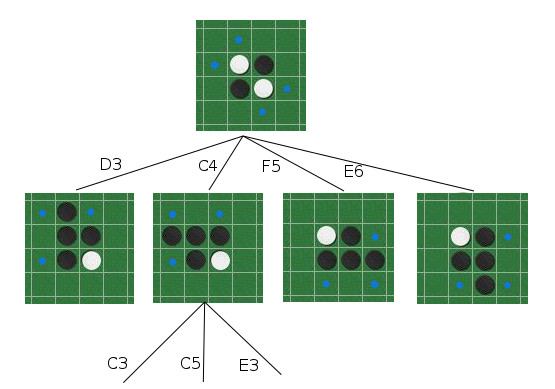
\includegraphics[scale=0.6]{exemple_arbre.jpg}
\centering
\caption{Exemple d'arbre que l'on peut générer. A partir de la position de départ du jeu, les sommets de l'arbre sont les états et les chemins des coups possibles.}
\end{figure}

Même si le \textit{Reversi} sur un plateau de 8x8 n'a pas encore été résolu, des solutions ont été trouvées pour des parties en 4x4 et 6x6\cite{sol6x6}.

Afin de trouver rapidement le meilleur coup (celui qui donne le plus de chance de gagner la partie), les programmes ont besoin dans un premier temps d'une technique de parcours d'arbre efficace, mais aussi d'heuristique. De nombreuses techniques de parcours existent, parmi les plus utilisées on peut citer:
\begin{itemize}
\item \textit{Minimax Alpha-beta pruning}\cite{alpha-beta}, le grand avantage de cette méthode est qu'elle élimine des branches au fur et à mesure de son déroulement. Elle est donc assez optimisée pour les arbres représentants les coups possibles d'un jeu de plateau.
\item \textit{Negamax} Une variante simplifiée de minimax, lors du calcul de la perte maximum on part du principe que la valeur d'un coup pour un joueur donné est égale à la négation de la valeur de l'autre joueur. Ainsi au lieu de calculer le minimum et maximum pour chaque joueur et chaque coup on dit que \begin{math}
max(a, b) == -min(-a, -b).
\end{math}
\end{itemize}

Comme dit précédemment, on ne sait pas, à l'heure actuelle, aller jusqu'au bout de l'arbre des coups possibles, c'est pour cette raison que nous avons besoin d'une fonction d'évaluation. Le but de cette fonction est d'attribuer une valeur au sommet représentant les états du jeu. Plusieurs techniques sont possibles\cite{heuristique}.
\begin{itemize}
\item IAGO: Cette méthode consiste à utiliser les connaissances que l'on a du jeu de Reversi\cite{strategie}, en effet on peut dégager des critères augmentant les chances de gagner. Par exemple les bords et les coins sont des positions très intéressantes à avoir car elles sont difficiles ou impossibles à retourner. En réduisant le nombre de coups possibles pour l'adversaire on peut aussi l'obliger à jouer des coups nous favorisant (par exemple nous permettre de prendre possession d'un coin). En étant capable d'extraire ces informations on peut évaluer chaque coup.
\item LOGISTELLO: La méthode utilisée par le programme ayant battu le champion du monde se base sur des parties jouées. En faisant analyser les coups joués et le résultat de la partie à un ordinateur on peut obtenir une heuristique basée sur des parties réelles plutôt que deviner les éléments importants pour gagner.
\end{itemize}

Enfin, afin de représenter le plateau d'une façon permettant des manipulations rapides, une structure spécifique a été inventée: les Bitboards\cite{bitboard}. Cette structure de données est un tableau de bit représentant la présence ou non des pions sur la case correspondante. Le principal avantage de cette stucture est qu'elle permet la manipulation du plateau par des opérations bit à bit, opérations pouvant être effectuées très rapidement par les processeurs. Le deuxième avantage est que cette information prend très peu de place en mémoire. Dans le cas du Reversi, le plateau peut être représenté par deux bitboards, un codant les positions des pions blancs et l'autre les positions des pions noirs.

\section{Description des besoins}
\subsection{Fonctionnels}

\subsubsection{Liste des besoins liés à la simulation de jeu :}

\textbf{Déterminer les coups possibles à jouer :}
Dans les règles du Reversi\cite{regle}, peu ou aucun coups sont possibles à chaque tour, nous devons donc pouvoir les déterminer pour respecter les règles du jeu et pour savoir si le coup qui est demandé est légal ou non.

\textbf{Actualiser le plateau après un coup :}
Lorsque l'on rajoute un pion au plateau il faut changer la couleur des pions qui ont été capturés avant de changer de joueur.

\textbf{Reconnaître une fin de partie : }
Pour savoir quand arrêter le jeu nous devons reconnaître une fin de partie. Il n'y a soit plus de case libre soit plus de coups légaux disponibles pour les deux joueurs.

\subsubsection{Liste des besoins liés à l'interface utilisateur :}

\textbf{Démarrer une partie :}
Au lancement du programme il faut qu'une partie se lance selon les paramètres passés par l'utilisateur, ces options permettront de:
\begin{itemize}
\item spécifier la taille
\item reprendre une partie sauvegardée dans un fichier texte
\item faire jouer les blancs et/ou noir par une IA
\item lancer le mode contest
\item afficher l'aide
\end{itemize}

\textbf{Afficher l'état de la partie sur la console :}
Il faut pouvoir afficher le plateau de jeu quelle que soit sa taille, en dessous d'une certaine limite, et d'une manière qui soit compréhensible par le joueur.

\textbf{Déterminer les coups possibles à jouer et les afficher:}
Il faut pouvoir prévoir les coups légaux qui permettent de prendre des pions à l'adversaire et les rajouter sur l’affichage, pour que le joueur puisse savoir où il a le droit de jouer.

\textbf{Choisir un coup:}
Le joueur doit pouvoir placer un pion, ce qui aura pour effet si le coup est légal, d'actualiser l’état de la partie, ou le cas échéant, de redemander une position au joueur.

\textbf{Finir une partie : }
La partie se terminera par un affichage des scores et la possibilité de recommencer une partie, ou d’arrêter le programme sera proposée au joueur.

\textbf{Sauvegarder une partie dans un fichier texte :} 
Si l'on souhaite continuer la partie plus tard, nous devons être capable de sauvegarder l'état actuel dans un simple fichier texte avant de fermer le programme. L'écriture de ce fichier doit respecter la syntaxe fixée par le client (Voir figure ~\ref{SaveExemple}) qui sera expliquée plus bas.

\textbf{Charger une partie à partir d'un fichier de sauvegarde :}
Une fois qu'une partie est sauvegardée, si l'on souhaite la continuer nous devons pouvoir placer en entrée de notre programme le nom d'un fichier de sauvegarde qui respecte la syntaxe (Voir figure ~\ref{SaveExemple}) et continuer la partie à partir de l'état de jeu actuel.

\textbf{Respecter la syntaxe du fichier de sauvegarde (voir ~\ref{SaveExemple}) pour que le programme arbitre du client puisse l'utiliser :}

\begin{itemize}
\item Les lignes vides, espaces et tabulation ne sont pas pris en compte, seuls les lignes non vides sont significatives.
\item La première ligne significative indique le joueur courant('X' pour le joueur noir et 'O' pour le joueur blanc).
\item Chaque lignes significatives qui suit représente une ligne du plateau, avec pour chaque case,'\_' si la case est vide, 'X' si il y a un pion noir et 'O' si il y a un pion blanc.
\item Chaque fin de ligne est défini par un '\textbackslash n'.
\item Le caractère '\#' indique un commentaire jusqu'au prochain '\textbackslash n'
\item Les lignes ne contenant que des commentaires sont donc des lignes considérées vides.
\item Il faut respecter des tailles carrées et paires tels que 2x2, 4x4, 6x6, 8x8...
\end{itemize}
\begin{figure}[H]

\begin{lstlisting}
		    X
		    _ _ _ _ _ _ _ _
		    _ _ _ _ _ _ _ _
		    _ _ _ _ _ _ _ _
		    _ _ _ X O _ _ _
		    _ _ _ O X _ _ _
		    _ _ _ _ _ _ _ _
		    _ _ _ _ _ _ _ _
		    _ _ _ _ _ _ _ _
		    #Plateau de depart
             
\end{lstlisting}
\caption[SaveExemple]
{Exemple fichier sauvegarde}
\label{SaveExemple}

\end{figure}

\textbf{Choisir la taille du plateau :}
On doit pouvoir choisir la taille du plateau de jeu, il faut cependant que  le plateau de jeu soit un carré de nombre pair pour que la partie soit jouable.

\textbf{Avoir un mode "Contest" :} 
Ce mode permettra au client d'utiliser notre intelligence artificielle au cours d'une partie. Il faut pouvoir prendre en entrée une partie en cours et afficher sur le terminal le coup que l'on souhaite jouer. Le client utilisera lui son programme arbitre pour faire jouer notre intelligence artificielle.


\subsubsection{Liste des besoins liés à l'intelligence artificielle :}
Pour réaliser notre intelligence artificielle, nous utiliserons des algorithmes de parcours d'arbres\cite{arbre} qui étudieront les différents coups possibles afin de choisir le meilleur. Il est donc nécessaire d'implémenter les besoins suivants :

\textbf{Créer les fils d'un nœud}
Chaque nœud de l'arbre se composera d'une configuration de jeu et du joueur qui devra jouer. Car une configuration de jeu seule ne permet pas de savoir quel joueur vient de jouer. Nous devons donc à partir d'un noeud, pouvoir déterminer tous ses fils (l'ensemble des coups qui suivront la configuration actuelle).

\textbf{Fixer une profondeur limite à notre arbre}
Il est impossible de générer entièrement l'arbre des coups possibles du Reversi, il est donc necessaire de fixer une limite à la profondeur de notre arbre si l'on souhaite le générer.

\textbf{Fusionner les branches identiques}
Des coups différents peuvent parfois mener à des configurations de jeux identiques ou symmétriques. Afin de limiter la taille de notre arbre, on peut les fusionner lorsqu'on les détecte.

\textbf{Parcourir notre arbre des coups}
Différentes techniques de parcours d'arbre existent, certaines ont besoin d'un arbre déjà créé (le Minimax\cite{minimax} par exemple), d'autres le construisent au fur et à mesure (alpha beta prunning\cite{alpha-beta} par exemple) afin d'éviter de créer les noeuds que l'on a pas besoin d'étudier. Nous devons les étudier pour trouver la performante.

\textbf{ Attribuer une valeur à une configuration de jeu}
Lorsque l'on parcourt notre arbre, nous devons attribuer à chaque état du jeu une valeur afin de pouvoir séléctionner le meilleur coup. Là encore, différentes techniques existent. Par exemple, le nombre de pions que l'on possède après un coup ou le nombre de coup différent que l'on pourra faire pour avoir plus de choix ou encore, le nombre de pions stables (qui ne peuvent pas être repris par le joueur adverse). Il nous faudra donc en implémenter plusieurs afin de les comparer et choisir la meilleure ou d'en utiliser plusieurs.

\subsection{Non fonctionnels}
\begin{itemize}
\item Utilisation de deux bitboards\cite{introbitboard} pour représenter les pions noirs et blancs
\item Actualisation de l'affichage en moins d'une seconde
\item IA suffisamment rapide (10 secondes sur les ordinateurs du Crémi)
\end{itemize}


\begin{figure}[H]
\begin{tikzpicture}[node distance=2.5cm,auto,>=stealth']

	%Nom en haut
    \node[] (utilisateur) {utilisateur};
    \node[right = of utilisateur] (interface) {interface};
    \node[right = of interface] (jeu) {jeu};
    \node[right = of jeu] (IA) {IA};
    
    
  	%Trait vertical
    \node[below of=utilisateur, node distance=12cm] (utilisateur_ground) {};
    \node[below of=interface, node distance=12cm] (interface_ground) {};
    \node[below of=jeu, node distance=12cm] (jeu_ground) {};
    \node[below of=IA, node distance=12cm] (IA_ground) {};
    
    \draw (utilisateur) -- (utilisateur_ground);
    \draw (interface) -- (interface_ground);
    \draw (jeu) -- (jeu_ground);
    \draw (IA) -- (IA_ground);
    
    %Ligne
    \draw[->] ($(utilisateur)!0.08!(utilisateur_ground)$) -- node[above,scale=0.8,midway]{Demande l'affichage} node[below,scale=0.8,midway]{du plateau} ($(interface)!0.08!(interface_ground)$);
    \draw[->] ($(interface)!0.15!(interface_ground)$) -- node[above,scale=0.8,midway]{Demande la position} node[below,scale=0.8,midway]{des pions} ($(jeu)!0.15!(jeu_ground)$);
    \draw[<-] ($(interface)!0.25!(interface_ground)$) -- node[above,scale=0.8,midway]{Renvoie la position}node[below,scale=0.8,midway]{des pions actuels} ($(jeu)!0.25!(jeu_ground)$);
    \draw[<-] ($(utilisateur)!0.32!(utilisateur_ground)$) -- node[above,scale=0.8,midway]{Affiche le plateau}node[below,scale=0.8,midway]{et attend le coup} ($(interface)!0.32!(interface_ground)$);
    \draw[->] ($(utilisateur)!0.42!(utilisateur_ground)$) -- node[above,scale=0.8,midway]{Rentre le coup}($(jeu)!0.42!(jeu_ground)$);
    \draw[<-] ($(utilisateur)!0.50!(utilisateur_ground)$) -- node[above,scale=0.8,midway]{Coup non OK}node[below,scale=0.8,midway]{redemande le coup}($(jeu)!0.50!(jeu_ground)$);
    \draw[->] ($(utilisateur)!0.60!(utilisateur_ground)$) -- node[above,scale=0.8,midway]{Rentre le coup}($(jeu)!0.60!(jeu_ground)$);
    \draw[<-] ($(interface)!0.68!(interface_ground)$) -- node[above,scale=0.8,midway]{Coup OK}($(jeu)!0.68!(jeu_ground)$);
    \draw[<-] ($(utilisateur)!0.76!(utilisateur_ground)$) -- node[above,scale=0.8,midway]{Actualise l'affichage}node[below,scale=0.8,midway]{et attend le coup} ($(interface)!0.76!(interface_ground)$);
    \draw[->] ($(jeu)!0.76!(jeu_ground)$) --
node[above,scale=0.8,midway]{Demande de coup}node[below,scale=0.8,midway]{} ($(IA)!0.76!(IA_ground)$);
	\draw[<-] ($(jeu)!0.84!(jeu_ground)$) -- node[above,scale=0.8,midway]{Rentre le coup}($(IA)!0.84!(IA_ground)$);
	\draw[<-] ($(interface)!0.91!(interface_ground)$) -- node[above,scale=0.8,midway]{Coup OK}($(jeu)!0.91!(jeu_ground)$);
    \draw[<-] ($(utilisateur)!0.97!(utilisateur_ground)$) -- node[above,scale=0.8,midway]{Actualise l'affichage}node[below,scale=0.8,midway]{et attend le coup} ($(interface)!0.97!(interface_ground)$);
    
    
\end{tikzpicture}
\caption{Diagramme de séquence du lancement du lancement du programme}
\end{figure}

\section{Diagramme de Gant}

\begin{ganttchart}[
vgrid,
title/.style={fill=teal, draw=none},
title label font=\color{white}\bfseries,
title left shift=.01,
title right shift=-.01,
title top shift=.0,
hgrid,
x unit=1mm,
time slot format=isodate,
today=2018-02-02,
progress=today,
bar/.append style={fill=green},
bar incomplete/.append style={fill=red},
group incomplete/.append style={draw=black,fill=none},
]{2018-02-01}{2018-04-30}
\gantttitle{Joueur de Reversi}{89} \\
\gantttitlecalendar{year,month=name} \\
\ganttgroup{Projet}{2018-02-02}{2018-04-05} \\
\ganttgroup{Release 1}{2018-02-02}{2018-02-16} \\
\ganttgroup{Release Finale}{2018-02-16}{2018-04-05} \\
\ganttbar{Simulation de jeu}{2018-02-02}{2018-02-16} \\
\ganttbar{Interface utilisateur}{2018-02-02}{2018-02-16} \\
\ganttgroup{Développement IA}{2018-02-02}{2018-04-05} \\
\ganttbar{Premiere IA Basique}{2018-02-02}{2018-02-16} \\
\ganttbar{IA Avancé}{2018-02-16}{2018-04-05} \\


\end{ganttchart}

\section{Bibliographie}

\bibliographystyle{unsrt}
\bibliography{biblio}
\end{document}